\graphicspath{{chapters/chapter4/imgs/}}

\chapter{Sposoby generowania narracji}\label{chapter:ch4}

W poprzednich sekcjach omówiona została historia oraz wykorzystywane w grach komputerowych rodzaje
narracji. W każdym z tych elementów istnieje jeden element wspólny: to ludzie odpowiadają za tworzenie
narracji, odpowiednie jej planowanie i prezentowanie odbiorcy. Związane z tym są oczywiście olbrzymie
koszty oraz duży nakład czasu poświęcony przez pracowników. Biorąc pod uwagę terminy stale goniące
producentów gier, nic dziwnego, że pewne zaplanowane fragmenty fabularne nie znajdują miejsca w~końcowym
produkcie. Z tego względu, patrząc na postępujący rozwój technologiczny, nasuwa się pytanie ---
czy da się zarządzać narracją w grze komputerowej w sposób automatyczny? W ramach tej sekcji
przedstawione zostaną znane rozwiązania z dziedziny sztucznej inteligencji pomagające w kreowaniu fabuły
oraz nakreślony zostanie potencjał w tej sferze dużych modeli językowych.

\section{Wykorzystanie algorytmów sztucznej inteligencji do kreowania narracji}\label{section:ch4_1}

Mówiąc o ogólnym wykorzystaniu algorytmów sztucznej inteligencji można cofnąć się do bardzo prostych
rozwiązań wykorzystanych np. w "Pong" (Patrz sekcja \ref{subsection:ch1_2}), do technik generowania
proceduralnego (zwłaszcza poziomów) czy też do systemów rankingowych (np. system TrueSkill). Jako, że
nie są to metody stricte powiązane z narracją to nie zostaną one opisane bardziej szczegółowo.
Przedstawione natomiast będą kluczowe obszary wykorzystywane w grach: częściowo-uporządkowane planowanie
(ang. \textit{\gls{pop}} - partially-ordered planning), modelowanie doświadczeń gracza (ang. \textit{\gls{pem}} -
player experience modelling), przetwarzanie języka naturalnego (ang. \textit{\gls{nlp}} - natural language
processing), postać niegrywalna (ang. \textit{\gls{npc}} - non-playable character), proces decyzyjny Markowa
(ang. \textit{\gls{mdp}} - Markov decision process).

\subsubsection*{POP (Partially-ordered planning)}

Planowanie częściowo-uporządkowane jest skierowanym grafym acyklicznym, gdzie węzły są operacjami
(inaczej nazywanymi akcjami), które po wywołaniu zmieniają stan świata. Krawędzie przedstawiają
relacje przyczynowe i czasowe pomiędzy akcjami. Powiązanie przyczynowe $a_{i} \rightarrow^{c}a_{j}$
oznacza, że wykonanie akcji $a_{i}$ zmieni stan warunku $c$ na prawdziwy w świecie fabuły, a co za
tym idzie akcja $a_{j}$ zależna od tego warunku będzie możliwa do wykonania. Powiązanie czasowe
przedstawia ograniczenie porządkowe pomiędzy operacjami, gdzie jedna operacja musi być wykonana przed
inną\cite{game_ai_storytelling}. Przykładowa struktura fabularna zrealizowana za pomocą planowania
częściowo-uporządkowanego została przedstawiona na rysunku \ref{fig:ch4_1_pop}.

\begin{figure}[h]
    \centering
    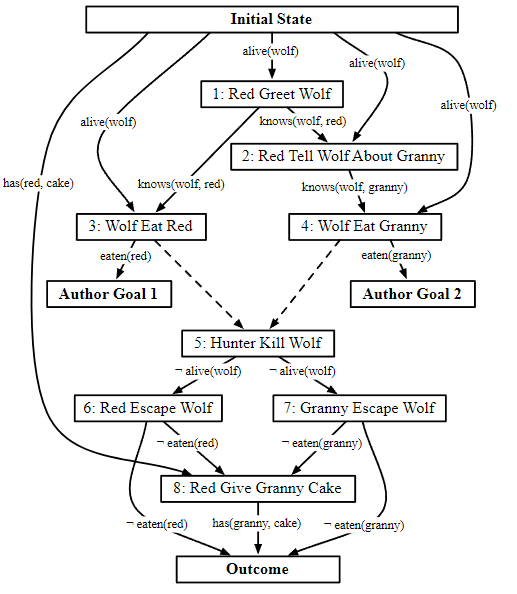
\includegraphics[width=0.5\textwidth]{ch4_1_pop.png}
    \caption{Fabuła "Czerwonego Kapturka" zapisana za pomocą POP}
    \label{fig:ch4_1_pop}
\end{figure}

Za pomocą tej techniki kreować można rozbudowane plany fabularne, które mogą ulegać zmianie na
podstawie akcji podejmowanych przez gracza czy zmian zachodzących w~świecie gry. Odpowiednie algorytmy
przeszukiwania nazywane \textit{"plannerami"} rozwiązują problem planowania, tzn. mając dany stan
świata, pewne atomowe akcje możliwe do wykonania przez grającego oraz założony cel, znajdują
odpowiednią sekwencję operacji, które doprowadzą do osięgnięcia tegoż celu\cite{game_ai_storytelling}.

Podstawowym problemem pojawiającym się przy wykorzystaniu metody \gls{pop} jest to, że zarówno gracz jak i
potencjalnie inne niegrywalne postacie, mogą być zdolne do wywołania akcji w świecie gry, która
zagraża dalszemu przebiegowi fabularnemu zgodnego z planem\cite{characters_and_directors}. Wtedy
stosowane są odpowiednie techniki naprawcze, które prowadzą do mniej lub bardziej doskonałych rozwiązań.

\subsubsection*{PEM (Player experience modelling)}

Modelowanie doświadczeń gracza polega na zbieraniu danych behawioralnych czy też wydajnościowych
(punkty, czas, decyzje) ze względu na rozgrywkę za pomocą wielu modalności: mowy gracza, obrazów
(śledzenie ruchów ciała, mimiki twarzy, gałek ocznych) czy też sygnałów fizjologicznych (puls czy
przewodność skóry). Pomiar sygnałów fizjologicznych jest oczywiście problematyczny ze względu na
wykorzystanie dodatkowego sprzętu a zarazem inwazyjność przeszkadzającą w swobodnej rozgrywce
\cite{reusable_game_ai}.

W ramach tego obszaru sztuczna inteligencja objawia się zazwyczaj pod postacią sieci neuronowych czy
też drzew decyzyjnych, które pozwalają dokonywać klasyfikacji w~zakresie\cite{reusable_game_ai}:

\begin{itemize}
    \item rozpoznawania emocji grającego - w ramach anagażujących systemów dialogowych
    \item balansowania rozgrywki - tak by gracz nie odczuwał frustracji ze względu na zbyt wysoki poziom
          trudności a zarazem by nie doznawał nudy ze względu na zbyt prostą rozgrywkę
    \item oceniania umiejętności gracza - do prowadzenia badań w sposób ukryty
\end{itemize}

\subsubsection*{NLP (Natural language processing)}

Przetwarzanie języka naturalnego jest dziedziną w obrębie sztucznej inteligencji, która zajmuje się
zrozumieniem, interpretacją i manipulacją ludzkiego języka\cite{reusable_game_ai}. W ramach gier
komputerowych pozwala to graczowi poruszać się po świecie czy też komunikować z~innymi postaciami \gls{npc}
w sposób zarówno naturalny (zamiast wchodzenia w interakcję z odpowiednimi interfejsami) jak i dość
otwarty (na tyle na ile dany system jest w stanie przetwarzać odpowiednie frazy).

Z podstaw przetwarzania języka naturalnego korzystały tytuły realizowane w konwencji interaktywnej
fikcji, takie jak "Otchłań" (Patrz sekcja \ref{subsection:ch3_2}). Pozwalają one graczowi za pomocą
określonego zestawu komend poruszać się i wchodzić w interakcję z całym światem gry.

Związane z tą dziedziną są duże modele językowe, które potrafią operować językiem naturalnym.
Ich bardziej szczegółowy opis będzie przedstawiony w sekcji \ref{section:ch4_2}.

\subsubsection*{NPC (Non-playable character)}

Postacie niegrywalne to wszelkie jednostki czy postacie, z którymi gracz może wchodzić w
interakcję lub dostrzegać ich autonomiczne poruszanie w świecie. Mogą to być statyczne byty,
które usytuowane są w jednym określonym miejscu i mają na celu dawać grającemu zadania czy też
informacje o świecie gry. Z drugiej strony wszelkie jednostki, z~którymi gracz walczy również
podlegają pod tę definicję. Forma postaci niegrywalnych, tak jak i w literaturze, nie jest
istotna, gdyż bohaterem może być zarówno człowiek jak i~zantropomorfizowane zwierzę czy rzecz.

\gls{npc} pojawiły się w grach z początkiem lat 90-tych. Oparte były przede wszystkim na zpredefiniowanych
skryptach i drzewach decyzyjnych\cite{storytelling_through} (współcześnie nadal wiele postaci jest
opartych o te rozwiązania)\cite{from_pong_to_narrative}.

Wraz z rozwojem technologicznym twórcy gry mają możliwość przeznaczenia więcej mocy obliczeniowej
na wiarygodne dla gracza postacie \gls{npc}. Związane jest to z dokładniejszymi modelami i animacjami
postaci ale również z bardziej zaawansowanymi wzorcami zachowania. Producenci zaczęli wykorzystywać
od lat 2010 w tym celu techniki uczenia maszynowego oraz głębokiego nauczania
\cite{from_pong_to_narrative}. Pozwala to przeciwnikom (czy też sprzymierzeńcom) gracza
dostosowywać się do sposobu prowadzenia przez niego rozgrywki. Współczesne tytuły takie jak
"Read Dead Redemption 2" czy "The Last of Us Part II" wykorzystują głębokie sieci neuronowe do
budowania postaci \gls{npc}\cite{from_pong_to_narrative}.

\subsubsection*{MDP (Markov decision process)}

Łańcuch Markowa jest stochastycznym modelem opisującym ciąg możliwych zdarzeń, w którym
prawdopodobieństwo każdego zdarzenia zależy jedynie od wyniku poprzedniego. Rozróżniane one
są dodatkowo ze względu na dyskretne lub ciągłe momenty czasowe, w których następuje zmiana
stanów. Proces decyzyjny Markowa (\gls{mdp}) jest zasadniczo rozszerzeniem łańcuchów Markowa ---
różnicę stanowi dodanie akcji (które pozwalają na podejmowanie decyzji) oraz nagród otrzymywanych
po przejściu z jednego stan w drugi. Jeżeli dla każdego stanu istnieje tylko jedna akcja i
wszystkie nagrody są jednakowe, to proces decyzyjny Markowa upraszcza się do łańcucha Markowa.

\begin{figure}[h]
    \centering
    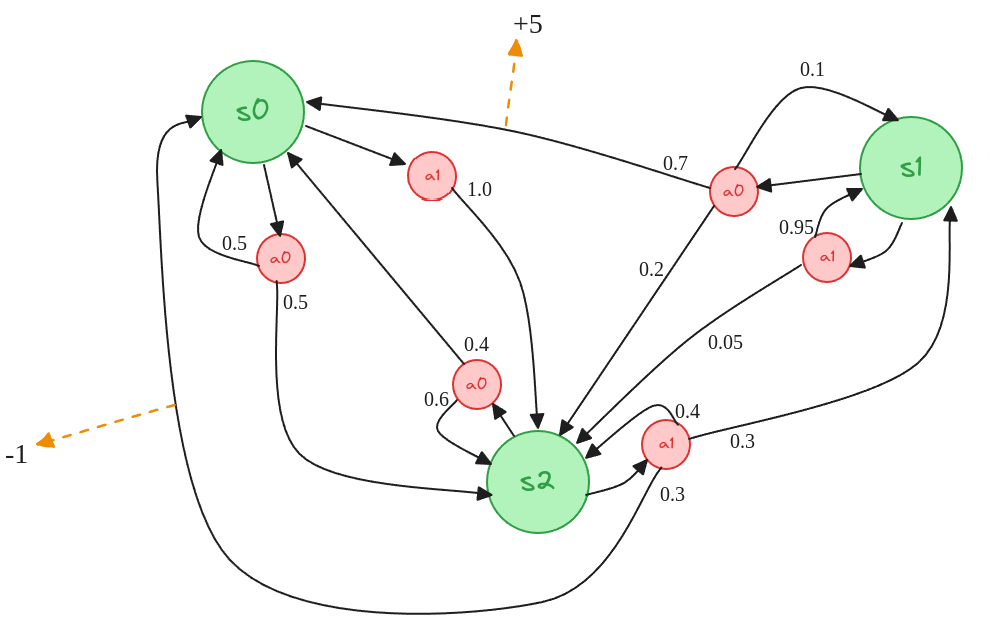
\includegraphics[width=0.8\textwidth]{ch4_1_mdp.png}
    \caption{Przykładowy proces decyzyjny Markowa}
    \label{fig:ch4_1_mdp}
\end{figure}

Na powyższym rysunku przedstawiony został przykładowy proces decyzjny Markowa z~trzema stanami (zielone
kółka), dwiema akcjami (czerwone kółka) oraz dwiema nagrodami (pomarańczowe strzałki). Model \gls{mdp} może
być wykorzystany w ramach generowania treści gier komputerowych do budowania zadań dla gracza,
przykładowo dla gry kucharskiej baza składników może być ułożona w odpowiednie łańcuchy Markowa, tak
by bardziej pasujące do siebie składniki miały większe prawdopodobieństwo bycia wspólnie wybranym
\cite{ammanabrolu2020automated}.

Proces może być dodatkowo wykorzystany w proceduralnym generowaniu treści czy świata dla gracza.
Zakładając, że to gracz jest \textit{"agentem"} podejmującym akcje w świecie gry (które są jawnie
zdefiniowane przez twórców), doprowadza on do zmiany stanu świata co jest idealnie reprezentowane
przez proces decyzyjny Markowa\cite{automated_planning}.

\subsubsection*{Przykład wykorzystania - "Façade"}

"Façade" (2005) to tytuł, który próbował złamać znany do tamtej pory podział na narrację liniową czy też
rozgałęziającą się, na rzecz w pełni interaktywnej historii kontrolowanej przez gracza. Jest to
trójwymiarowa gra czasu rzeczywistego przedstawiona w formie jednego aktu. Narracja koncentruje się
wokół Grace i Tripa, małżeństwa po trzydziestce, które zaprasza gracza na drinka. Gracz nie wie, że ich
małżeństwo znajduje się na grząskim gruncie, a tego wieczoru wszystkie ich małżeńskie problemy wyjdą na
jaw. To, w jaki sposób ich związek się rozpadnie, a także ostateczny związek gracza z Grace i Tripem,
zależy od interakcji gracza ze światem. Gracz angażuje się poprzez poruszanie się po środowisku,
manipulowanie przedmiotami i, co najważniejsze, poprzez dialogi w języku naturalnym\cite{1024751}.

Twórcy na potrzebę "Façade" stworzyli własny język ABL (\textit{"A Behavior Language"} - z~ang. język
zachowań). Stanowi on pewnego rodzaju połączenie drzew decyzjnych i~procesów decyzjnych Markowa
wspomnianych wcześniej. Programy ABL są zorganizowane jako zbiór zachowań, które mogą być procesowane
sekwencyjnie lub równolegle. Dodatkowo, zachowania mogą mieć narzucone określone wymagania by
mogły one się odbyć, a w~zależności od powodzenia lub porażki w realizacji zachowania świat gry
może zostać odpowiednio zmieniony.

\section{Wykorzystanie dużych modeli językowych (LLM) do kreowania narracji}\label{section:ch4_2}

W ostatnich latach coraz większa liczba prac naukowych oraz rozwiązań komercyjnych skupia się wokół
tzw. dużych modeli językowych. Okazuje się bowiem, że wprowadzając optymalizacje w sferze oprogramowania
czy też po prostu przeznaczając więcej mocy obliczeniowej na wyuczenie takowych modeli, zyskuje się
adekwatnie większą \textit{"skuteczność"} jeżeli chodzi o wykonywane przez nie zadania z zakresu
przetwarzania języka naturalnego (i nie tylko!).

W związku z tym nasuwa się następujące pytanie --- czy można wykorzystać \textbf{aktualne} duże modele
językowe do skutecznego kreowania narracji? W ramach tej sekcji przedstawiona zostanie dokładniejsza
charakterystyka tych modeli a zarazem istniejące próby ich wykorzystania.

\subsubsection*{Definicja i charakterystyka dużych modeli językowych}

Duże modele językowe są modelami nauczania maszynowego, które są w stanie wykonywać zadania z dziedziny
przetwarzania języka naturalnego, takie jak generowanie tekstu, tłumaczenie tekstu z jednego języka
na inny czy prowadzenie rozmowy z człowiekiem w sposób konwersacyjny\cite{larp_language}. Pojęcie
"duże" oznacza w tym przypadku zarówno skalę samych modeli (miliardy czy biliony parametrów) jak i
wymaganą do ich wyuczenia ilość danych. Pojęcie \gls{llm} skoncentrowane jest zasadniczo wokół funkcjonalności
danego modelu, niezależnie od przyjętej do jego wyuczenia architektury.

Z uwagi na fakt, że zdecydowana większość modeli oparta jest na architekturze transformera to zostanie
ona krótko nakreślona. Dane podawane na wejście do modelu mogą być różnych modalności np. tekst,
audio czy obraz. Następnie, dane te dzielone są na tzw. żetony (ang. \textit{tokens}) - fragmenty tekstu,
obrazu lub dźwięku. Każdy żeton jest kodowany jako wielowymiarowy wektor liczbowy, odzwierciedlający
jego semantyczne właściwości. Następnie sekwencja wektorów przechodzi przez blok uwagi (ang.
\textit{attention}), gdzie wektory wzajemnie się aktualizują (ponieważ np. znaczenie słowa zależy od
kontekstu, czyli od słów występujących dookoła niego). Ten proces pozwala na lepsze zrozumienie
zależności pomiędzy elementami wejściowymi. Po bloku uwagi, wektory są przetwarzane przez
perceptron wielowarstwowy (ang. \textit{MLP - multi-layer perceptron}). Cykl bloków uwagi i~MLP jest
wielokrotnie powtarzany. Na końcu procesu otrzymujemy pojedynczą macierz, na podstawie której, poprzez
operację softmax, generowany jest rozkład prawdopodobieństwa dla możliwych żetonów następujących po
danym fragmencie wejściowym. Autorzy raportu technicznego dotyczącego \gls{gpt}-4 zauważają, że:

\begin{quote}
    \textit{"...Takie modele są ważnym obszarem badań, ponieważ mają potencjał do wykorzystania w szerokim
        zakresie zastosowań, takich jak systemy dialogowe"}\cite{openai2024gpt4}
\end{quote}

Można również wnioskować, że następne iteracje modeli będą coraz lepsze:

\begin{quote}
    \textit{"Jednym z głównych celów rozwoju takich modeli jest poprawa ich zdolności do rozumienia i
        generowania tekstu w języku naturalnym, szczególnie w bardziej złożonych i zniuansowanych
        scenariuszach."}\cite{openai2024gpt4}
\end{quote}

Wymienione są jednak przez autorów ograniczenia aktualnych modeli językowych, które uniemożliwiają ich
masową adopcję w wielu przestrzeniach:

\begin{quote}
    \textit{"Pomimo swoich możliwości, \gls{gpt}-4 ma podobne ograniczenia do wcześniejszych modeli \gls{gpt}: nie jest w
        pełni niezawodny (np. może cierpieć na „halucynacje”), ma ograniczone okno kontekstowe i nie uczy
        się na podstawie doświadczenia. Należy zachować ostrożność podczas korzystania z wyników \gls{gpt}-4,
        szczególnie w kontekstach, w których ważna jest niezawodność."}\cite{openai2024gpt4}
\end{quote}

Pod pojęciem "halucynacji" rozumiane jest wymyślanie faktów, ponieważ modele te same w sobie nie posiadają
żadnej podpiętej bazy wiedzy a generowany przez nie tekst wynika z modelu probabilistycznego (co nie
znaczy, że w ogólnie nie dysponują wiedzą). Wielkość okna kontekstowego oznacza na jakim rozmiarze
danych / żetonów model jest w~stanie jednocześnie pracować (tzn. w przypadku bardzo długich konwersacji
czy plików model może nie brać pod uwagę wczesnych informacji przy udzielaniu odpowiedzi).

\subsubsection*{Przykłady zastosowania dużych modeli językowych}

W badaniu Schaap i innych (2023)\cite{questville} zbadano potencjał modeli BERT i \gls{gpt}-2
do proceduralnego generowania zadań (questów) w grze QuestVille. Podejście
to polegało na połączeniu dwóch modeli językowych: BERT i \gls{gpt}-2 w sekwencji. Najpierw zdefiniowano krótkie
zdania będące podstawowymi zadaniami, z jednym słowem zamaskowanym. Zdania te przesyłano do modelu
BERT, który przewidywał najbardziej prawdopodobne słowa pasujące do kontekstu. Następnie losowo wybierano
jedno ze zwróconych słów i umieszczano je w zdaniu, tworząc wejście dla modelu \gls{gpt}-2. Model ten generował
dodatkowy tekst narracyjny uzupełniający podstawowe zadanie o motywacje, opis sytuacji i~wprowadzał
elementy fabularne. Wyniki sugerują, że takie połączenie modeli ma potencjał do generowania angażujących
zadań z narracją, bardziej wciągających niż podstawowe polecenia. Poprzedzanie wejść relacjami
między postaciami niegrywalnymi w grze kierowało generowaną treść w odpowiedni kontekst. Jednak
generowane zdania nie zawsze były w pełni spójne i odpowiednie. Autorzy uznali, że dalsze postępy w
dziedzinie \gls{nlp}, w~tym pojawienie się nowszych, lepszych modeli, mogą doprowadzić do jeszcze lepszych
rezultatów w przyszłości.\cite{questville}

Jak wskazują w swojej pracy Umbraško i Drury (2023)\cite{chatgpt_narrative},
duże modele językowe mogą odgrywać kluczową rolę w
dynamicznym tworzeniu treści gry na podstawie wejściowych danych tekstowych i kontekstu rozgrywki.
Opisany prototyp gry wykorzystuje interfejs \gls{api} ChatGPT do generowania początkowej sceny narracyjnej oraz
opisu przeciwników (orków) na podstawie wysłanego do modelu żądania w formacie \gls{json}. Kluczowym
elementem jest też dynamiczne tworzenie dalszych fragmentów narracji na podstawie działań gracza i~stanu
gry, w tym cech przypisanych wrogom (np. "płonący", "pijany"). Wprowadzanie tych cech jako danych
wejściowych pozwala modelowi językowemu na bardziej kontekstowe dopasowanie narracji.
Autorzy prototypu zdecydowali się na ograniczenie zakresu możliwych wyjść modelu (np. rodzaje broni
wrogów) dla zachowania spójności z mechanicznymi elementami gry. Wskazuje to na konieczność znalezienia
właściwej równowagi pomiędzy swobodą generatywną modelu a wymogami spójnego i czytelnego doświadczenia.
Wyzwaniem opisanym w pracy było zmapowanie całego stanu gry, takiego jak pozycje postaci, jako danych
wejściowych do modelu ChatGPT. Ostatecznie autorzy zdecydowali się na prostszy model, w którym tylko
kluczowe elementy stanu gry są przekazywane do generowania narracji. Zaprezentowany
prototyp stanowi ciekawą próbę praktycznego wykorzystania dużych modeli językowych do tworzenia
angażującej, interaktywnej narracji w grze wideo w oparciu o działania gracza. Pokazuje zarówno
obiecujące możliwości, jak i obecne ograniczenia takiego podejścia.\cite{chatgpt_narrative}

W pracy "LARP: Language-Agent Role Play for Open-World Games" (2023)\cite{larp_language} autorzy
proponują wykorzystanie dużych modeli językowych jako podstawę pod generatywnych agentów
występujących w środowiskach otwartych światów gier fabularnych. Kluczowym elementem architektury
zaproponowanej w pracy jest kognitywna architektura agenta inspirowana psychologią poznawczą. Składa
się ona z modułów odpowiedzialnych za pamięć długotrwałą, roboczą, przetwarzanie pamięci oraz
podejmowanie decyzji. Pozwala to na symulację ludzkich procesów poznawczych, takich jak kodowanie,
przechowywanie i przypominanie informacji z pamięci, a także rekonstrukcję zdarzeń oraz zapominanie.
Integracja tych mechanizmów z \gls{llm} umożliwia agentowi prowadzenie spójnej, długoterminowej narracji w
otwartym świecie gry. Kolejnym istotnym aspektem jest moduł interakcji ze środowiskiem, który przekłada
decyzje agenta na konkretne działania w grze. Wykorzystuje on bibliotekę akcji podstawowych oraz generuje
nowe sekwencje akcji przy użyciu dopasowanego \gls{llm} w celu realizacji zamierzonych celów agenta. Ten proces
stale wzbogaca bibliotekę akcji o nowe schematy postępowania. Ponadto, praca zakłada implementację
mechanizmu dopasowywania różnorodnych osobowości i perspektyw dla agentów za pomocą zbioru
drobniejszych, wyspecjalizowanych modeli \gls{llm}. Pozwala to na generowanie narracji dostosowanych do
zróżnicowanych tożsamości, stylów językowych i postaw bohaterów niegrywalnych. Podejście LARP łączy
zaawansowane techniki przetwarzania języka naturalnego z inspiracjami z psychologii poznawczej w celu
umożliwienia generowania spójnych, długoterminowych narracji agentów w bogatych, otwartych światach gier
fabularnych\cite{larp_language}.

W ramach pracy "Generative Agents: Interactive Simulacra of Human Behavior" (2023)\cite{ai_town_ref} autorzy przedstawiają koncepcję
generatywnych agentów, które wykorzystują duże modele językowe do symulacji wiarygodnych zachowań
ludzkich. W porównaniu z poprzednią, ta prezentuje wnioski dotyczące faktycznej implementacji tej struktury.
Architektura agenta opiera się na trzech głównych komponentach: strumieniu pamięci, refleksji
i planowaniu. Strumień pamięci to moduł długoterminowej pamięci, który rejestruje doświadczenia agenta
w języku naturalnym. Refleksja pozwala agentowi na wyciąganie wniosków na wyższym poziomie abstrakcji,
co przekłada się na lepsze kierowanie jego zachowaniem. Planowanie to proces przekształcania tych
wniosków i aktualnego środowiska w wysokopoziomowe plany działań, które są następnie realizowane przez
agenta. Autorzy przeprowadzają dwie ewaluacje agentów generatywnych: kontrolowaną ewaluację indywidualnych
zachowań oraz kompleksową ewaluację interakcji między agentami w~otwartym środowisku przez dwa dni czasu gry.
W ewaluacji technicznej wykorzystują metodę "wywiadu" z agentem w języku naturalnym, aby zbadać jego zdolność
do pozostania w charakterze, pamiętania, planowania, reagowania i dokładnego refleksji. Porównują różne
wersje systemu z ograniczonym dostępem do pamięci, refleksji i planowania, obserwując, że każdy z tych
komponentów jest kluczowy dla wiarygodności zachowań agenta\cite{ai_town_ref}.

Jak widać obecnie trwają intensywne prace badawcze nad wykorzystaniem dużych modeli językowych,
w dziedzinie tworzenia treści literackich oraz elementów gier. Jednym z~obiecujących
zastosowań jest stworzenie w pełni autonomicznych, generatywnych agentów literackich,
zdolnych do samodzielnego tworzenia spójnych i angażujących narracji. Rozwiązania te stopniowo
znajdują swoje odzwierciedlenie również na rynku komercyjnym, czego przykładem są platformy takie
jak Inworld AI czy Nvidia Avatar Cloud Engine. Umożliwiają one twórcom gier, a nawet indywidualnym
użytkownikom, korzystanie z zaawansowanych modeli językowych w celu generowania dialogów postaci,
opisów środowisk czy całych wątków fabularnych. Chociaż wciąż istnieją liczne wyzwania natury
technicznej i etycznej, rozwój tej technologii może znacząco zmienić oblicze branży rozrywkowej
oraz procesów twórczych w dziedzinie literatury.